%begin-include

%In this chapter we present experiments of model selection of cell
% signaling pathways. We divide this chapter in two sections; the first
% section presents experiments to compare two model selection software: 
% ABC-SMC and SigNetMS, both of them presented on
% chapter~\ref{chap:model_selection_methods}. We end the first section
% presenting which software had best fit for our experiments. The
% following section presents experiments of model selection as a feature
% selection problem. We will analyze algorithm trace and what is the
% surface induced by the cost function over the search space.

\section{Choosing a Software for Model Selection}
% To choose a software for model selection we did the same experiment as
% girolami
%
% A simple instance of the model selection problem
% -> the correct model is...
% -> then we create other three models
%   - a simplification
%   - an overly complex model
%   - and an incorrect model
% -> the expected result for this experiment is that the correct model
%  has a higher (possibly be the first), and that the incorrect model
%  should be considered the worst. It is also important to see how the
%  software compares models with similar dynamics and with different
%  levels of complexity.
%  
% Results produced by SigNetMS and ABC-SysBio
% -> we proceeded to run both softwares 
% -> compare the ranking of both software
% -> show how the curve fits on both software
% -> show that there is some parameter value convergence on SigNetMS

To choose between SigNetMS and ABC-SysBio, we performed a model
selection experiment. This experiment, originally performed on the work
of Vyshemirsky and Girolami~\cite{Vyshemirsky2007}, consists in creating
artificial experimental data from a model of cell signaling pathway, and 
then selecting between four different models, including the correct one.
Using SigNetMS and ABC-SysBio we should be able to create a ranking of
the four models, in which we expect to see as the best, the model we
used to create the experimental data. More than that, we should analyze
the produced results to check if simpler models are preferred over
complex models; we should also check if the simulations produced by the
models, with the estimated sample of the posterior distribution of
parameters, approximates experimental data.

\subsection{A simple instance of the model selection problem}
\begin{figure}[h]
\begin{center}
    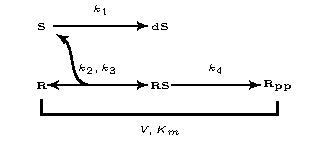
\includegraphics[width=.75\textwidth]{experiments/diagrams/bioinformatics_model1.pdf}
    \caption{A diagram that represents the correct model our simple
model selection experiment. This model represents a common motif, and
has S and Rpp as input and output, respectively. This model contains
five reactions: the decay of S to dS with $k_1$ as reaction rate
constant; the reversible reaction $\ce{S + R <=>[$k_1$][$k_2$] RS}$; the
first order reaction $\ce{RS ->[$k_4$] Rpp}$; and the Michaelis-Menten
reaction $\ce{A ->[$V, K_m$] B}$.}
    \label{fig:experiments:girolami_model1}
    \end{center}
\end{figure}

We start our model selection problem with the correct model, which is 
a signalling pathway composed by five reactions and five chemical 
species. Figure~\ref{fig:experiments:girolami_model1} shows a diagram
with this model. This model represents a common motif, and it has as the 
input signal the chemical species S, and as the output the chemical 
species Rpp; the experimental measurement used is the concentration of 
the output chemical species, which we donote as [Rpp].


In this experiment, for the sake of simplicity, we neglect the units of 
reaction rates constants and initial concentrations. The initial 
concentrations used are:  S $= 1$, R $= 1$, dS $= 0$, RS $= 0$, 
R$_{pp} = 0$. To create the experimental data, the reaction rate 
constants we used have the values: 
$k_1 = 0.07$, $k_2 = 0.6$, $k_3 = 0.05$, $k_4 = 0.3$, $V = 0.017$, and
$K_m = 0.3$. It is important to remember that we discard reaction rate
constant values during model selection; initial concentrations, however,
are still provided during this phase. To generate experimental data, we
simulate the dynamics of this model, using these parameter values, on
the time steps of: 2s, 10s, 20s, 40s, 60s and 100s. Three simulations
are created, and to each one of them we add, for each time measurement,
a Gaussian error with mean $0$ and standard deviation $0.01$. A
representation of the three experiment repetitions are showed on 
figure~\ref{fig:experiments:girolami_simulations}.

% TODO: determine the prior distribution used

% insert simulated data here
\begin{figure}
\begin{center}
    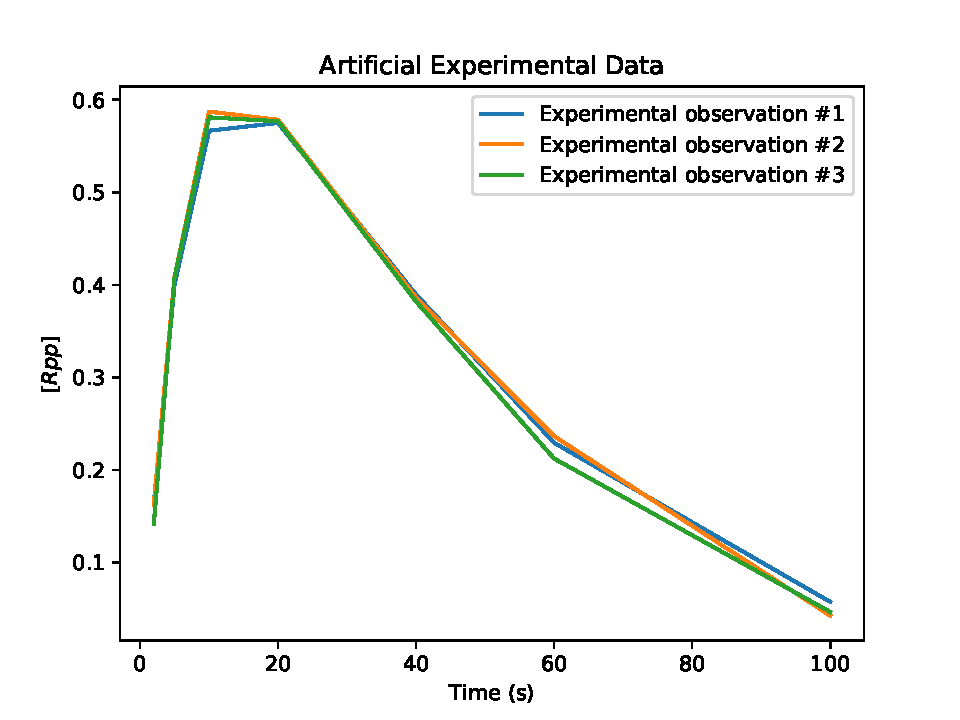
\includegraphics[width=.75\textwidth]{experiments/simulations/girolami_experimental_data.pdf}
    \caption{The dynamics produced by the correct model, with
pre-defined reaction rate constants plus a small Gaussian error, for
each time point. The measurement taken from the model is the
concentration of the Rpp species, which we denote as [Rpp]. We
linearly interpolate the experimental measure points to produce a
continuous dynamics from 2s to 100s.}
    \label{fig:experiments:girolami_simulations}
    \end{center}
\end{figure}

To assess the ranking produced by each of the model selection software,
we compare the first model with three other models (based on the correct
model): a simplified model; an overly simplified model, which should not 
be able to generate the observed dynamics; and, finally, a 
generalization (more complex) model.
Figure~\ref{fig:experiments:girolami_other_models} shows diagrams that
represent the three alternative models.

\begin{figure}[h]
    \centering
    \begin{tabular}{c c}
    \subfigure[simplified model]{
    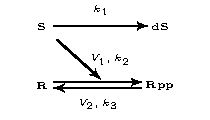
\includegraphics[clip=true,width=.45\linewidth]{experiments/diagrams/bioinformatics_model2.pdf}
    \label{fig:girolami_model2}}
    &
    \subfigure[overly simplified model]{
    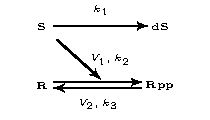
\includegraphics[clip=true,width=.45\linewidth]{experiments/diagrams/bioinformatics_model3.pdf}
    \label{fig:girolami_model3}} 
    \\
\multicolumn{2}{c}{    
    \subfigure[generalization model]{
    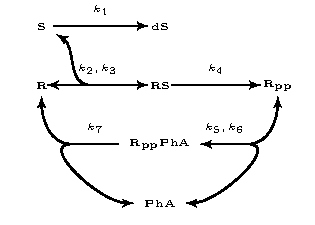
\includegraphics[clip=true,width=.45\linewidth]{experiments/diagrams/bioinformatics_model4.pdf}
    \label{fig:girolami_model4}}
} 
    \end{tabular}
    \caption{The diagrams of three other candidate models, based on the 
correct model that was presented before on 
Figure~\ref{fig:experiments:girolami_model1}. The 
model~\ref{fig:girolami_model2} is a simplification where we neglect the
chemical species RS, and we use the Michaelis-Menten to represent the
reaction $\ce{R -> Rpp}$ with S working as a catalyst.
Model~\ref{fig:girolami_model3} is the over simplified model, as it
neglects the decay of S; we do not expect this model to reproduce
experimental data, since the constant concentration level of S tend to
continuously produce Rpp, a species that, after 20 seconds, has a
monotonic decreasing concentration. Finally,
Model~\ref{fig:girolami_model4} is a generalization of the correct
model, as it generalizes the reaction $\ce{Rpp -> R}$, as instead of 
using the Michaelis-Menten kinetics, we use the enzymatic reaction 
$\ce{Rpp + PhA <=> RppPhA -> R + PhA}$; even though we expect this model
to be able to reproduce observed dynamics, we also expect that the
complexity of this model gets penalized.
}
    \label{fig:experiments:girolami_other_models}
\end{figure}

% -> the expected result for this experiment is that the correct model
%  has a higher (possibly be the first), and that the incorrect model
%  should be considered the worst. It is also important to see how the
%  software compares models with similar dynamics and with different
%  levels of complexity.

Before talking about results produced by different software, we should
note that this choice of candidate models are made so we can analyze
more than the ability of the software to correctly rank the correct
model as the best model. First, consider that we introduced a spurious
model, represented on figure~\ref{fig:girolami_model3} which neglects a
crucial reaction, making it impossible to reproduce the experimental
data; we expect this model to be ranked last between all models. Then,
there are two options to the correct model, one a simplification, and
the other a generalization. For these models, we expect that the
experimental dynamics are possible, however, we should be observant of
how they are ranked according to their complexity. That is important
because, one of the goals on using a Bayesian approach for model 
selection is that these approaches tend to automatically penalize overly
complex models.

% Comparing results of ABC-SMC and SigNetMS
\subsection{Solving a simple model selection instance using ABC-SysBio
and SigNetMS}
% What is the experiment
% What data the experiment produces;
% What are algorithm parameters we used;
% 1 - marginal likelihood of each model
% 2 - a sample of the posterior

% the input and output
After defining the candidate models and producing the artificial
experimental data, we proceeded to perform the experiment of model
selection. The instance related information provided to SigNetMS and 
ABC-SysBio is the same: a model, with predefined initial concentrations
of chemical species; a set of experiments, with the same time steps, 
with measurements of the concentration of Rpp; and a file containing
prior distributions for each one of the model parameters. It is
important to remember that the output produced by each software is
different. SigNetMS produces an estimative of $p({\bm D} | M)$ and also
a sample of the posterior distribution of parameters $p({\bm \theta} |
M, {\bm D})$ which is, in fact, composed by samples of all power
posterior distributions $p_{\beta}({\bm \theta})$ with values as we
described
on~\ref{sec:creating_an_estimative_of_the_marginal_likelihood}.
ABC-SysBio, on the other hand, produces an estimatives of $p({\bm
\theta}, M | {\bm D})$ that might be closer to this target distribution
on each iteration. Note that in this experiment, we need to run SigNetMS
for every model, while on ABC-SysBio we only need to run the software
once for all four candidate models.

The prior distribution of parameters are the same as used by Vyshemirsky
and Girolami~\cite{Vyshemirsky2007}. All model parameters priors are
Gamma(1, 3), where the first and second arguments are shape and scale. 
Gamma and Lognormal distributions are often used as prior for parameters 
because they have a zero probability density for negative values.
% what are algorithm parameter values used

For ABC-SysBio we decided to use its feature of automatically choosing
the schedule of threshold values, which is based on the acceptance of
produced individuals on each iteration. For SigNetMS, we used the
following parameters values: 15000 iterations of the naive burn-in, and
5000 iterations of the posterior shaped burn-in, with 1000 iterations
between covariation matrix rescales, and 3000 iterations of the
Populational MCMC. We used an empiric approach to determine these
parameter values, observing similar results when the number of
iterations are greater than these.

\subsubsection{The ranking produced by ABC-SysBio and SigNetMS}
The ABC-SysBio run created 26 populations of parameter values, each of 
them with 100 individual parameters values. At the last iteration, the 
algorithm stopped with $\epsilon = 1$ and the following estimates: 
\begin{itemize}
    \item{$\hat{p} (M = \text{Correct Model} | {\bm D}, \epsilon = 1) =
        0.005$;}
    \item{$\hat{p} (M = \text{Simplified Model} | {\bm D}, \epsilon = 1)
        = 0.014$;} 
    \item{$\hat{p} (M = \text{Incorrect Model} | {\bm D}, \epsilon = 1)
        = 0.976$;}
    \item{$\hat{p} (M = \text{Generalization Model} | {\bm D}, \epsilon
        = 1) = 0.003$.}
\end{itemize}
These estimates induces the ranking 3, 2, 1, 4.

After running the SigNetMS software four times, one for each model, we
were able to get the following estimates:
\begin{itemize}
    \item{$\log \hat{p}({\bm D} | M = \text{Correct Model}) = 26$}
    \item{$\log \hat{p}({\bm D} | M = \text{Simplified Model}) = 21$}
    \item{$\log \hat{p}({\bm D} | M = \text{Incorrect Model}) = -1$}
    \item{$\log \hat{p}({\bm D} | M = \text{Generalization Model}) =
        19$}
\end{itemize}

% subsubsection Comparing the produced ranking
\subsubsection{Comparing the ranking produced by ABC-SysBio and SigNetMS}
Before comparing the model ranking produced by ABC-SysBio and SigNetMS,
we should state that the ranking achieved by Vyshemirsky and 
Girolami~\cite{Vyshemirsky2007}, on the original work that introduced
this instance, is: Correct Model $\prec$ Generalization Model $\prec$
Simplified Model $\prec$ Incorrect Model. On this work, a methodology
similar to SigNetMS was used.

On ABC-SysBio results, we see that the Correct Model was not ranked
first, and, surprisingly, the Incorrect Model was ranked first. More
than that, when the algorithm stopped, other candidate models were
considered with low probability of being the ``true'' model, and
therefore we cannot strongly state a ranking between the other three
candidates.

On SigNetMS results, we see that the Correct Model was ranked first and 
the Incorrect Model is ranked last as expected. For these two models,
SigNetMS results are equal to the results of Girolami and Vyshemirsky,
and for the other two models, the ranking is the opposite. On SigNetMS,
we ranked the Simplified Model as better than the Generalization Model.
It is important to note here that, in fact, the Generalization Model,
which is more complex, was actually ranked worse than the Correct Model;
that is an evidence that this approach does penalize the complexity of
models.

% subsubsection Analyzing the distribution of posteriors
\subsubsection{Analyzing the posterior distributions produced by
ABC-SysBio and SignetMS}
If we consider only the ranking produced, there are indications that 
SigNetMS is a better choice for our application. However, we should also
take into account other output information produced by both software, 
relative to the distribution of model parameters. ABC-SysBio algorithm 
produces in every iteration a population of parameters that, when 
applied to an specific model, creates a simulation that is at most 
epsilon distant to the experimental measurements, with decreasing 
epsilon as the iteration number grows. SigNetMS, on the other hand, 
produces samples of forty power posterior distributions 
$p_\beta({\bm \theta})$, and although there is no threshold like there 
is on ABC-SysBio, we expect that the closer the value of $\beta$ is to 
$1$, the closer should be the produced simulation to the experimental 
measurements; this is explained by the fact that the power posterior 
distributions $p_0({\bm \theta})$ and $p_1({\bm \theta})$ are, 
respectively, the prior and posterior distribution of parameters.

% One way we could analyze data is looking at the produced simulations
A possible approach to analyze the produced parameters is to simulate
models with those parameter and create simulations to be compared with
the experimental measurements. For ABC-SysBio, in a population of 100
parameters, including the model indicator as one of the parameters, we
are able to simulate and visualize the generated experimental 
measurements for all individuals; on SigNetMS, on the other hand, the 
number of parameter values produced is much greater, than a randomly 
chosen subset of parameters should be enough. With such experiment, we 
are then able to identify what dynamics were created on the candidate 
models according to the estimated posterior distribution of parameters. 

On  figure~\ref{fig:girolami_allmodel_abc} we present the dynamics of 
sampled parameters of the last iterations of the ABC-SysBio run. We can
see on this figure that ABC-SysBio could not produce a set of parameter
values that allows the model to represent the dynamics observed on the
experiment. More than that, we can see that the incorrect model had the
best fit, and the dynamics produced by the sampled parameters induces a
nearly stationary dynamics of $[Rpp]$, with intermediary values of
concentration. With these results, we can understand that the ranking
produced by ABC-SysBio is incorrect because the software could not find
suitable parameter values that allow models to approximate the dynamics
observed on experiments.

\begin{figure}[ht]
    \centering
    \begin{tabular}{c c}
    \subfigure[correct model]{
    \includegraphics[clip=true,width=.45\linewidth]{experiments/abc_vs_snm/all_model/abc/msimulations_model1_25.pdf}
    \label{fig:girolami_model1_abc}}
    &
    \subfigure[simplified model]{
    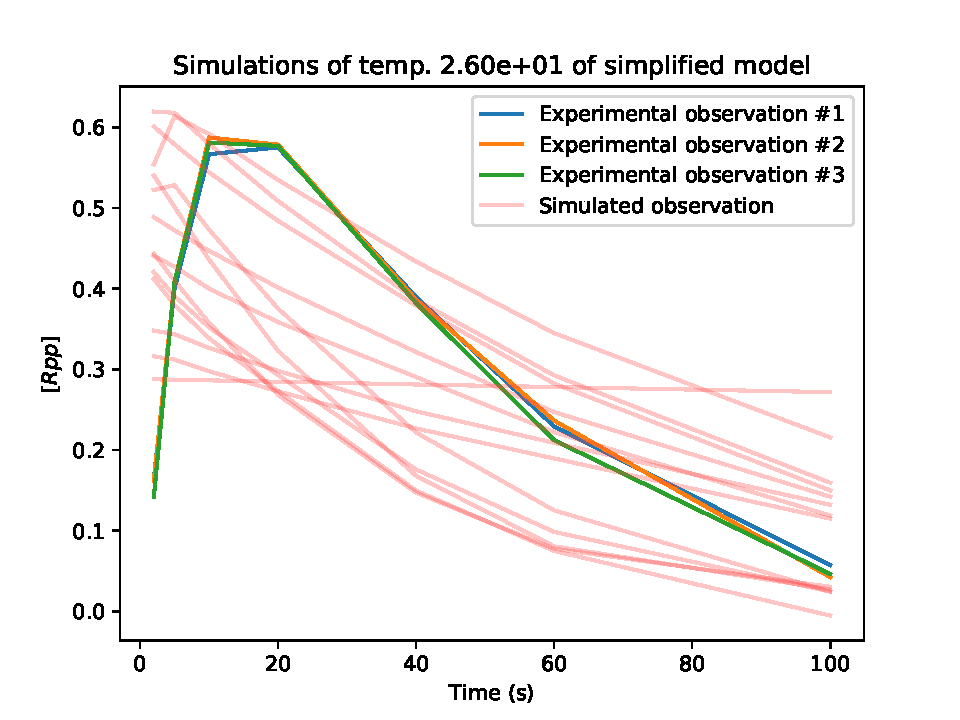
\includegraphics[clip=true,width=.45\linewidth]{experiments/abc_vs_snm/all_model/abc/msimulations_model2_25.pdf}
    \label{fig:girolami_model2_abc}} 
    \\
    \subfigure[incorrect model]{
    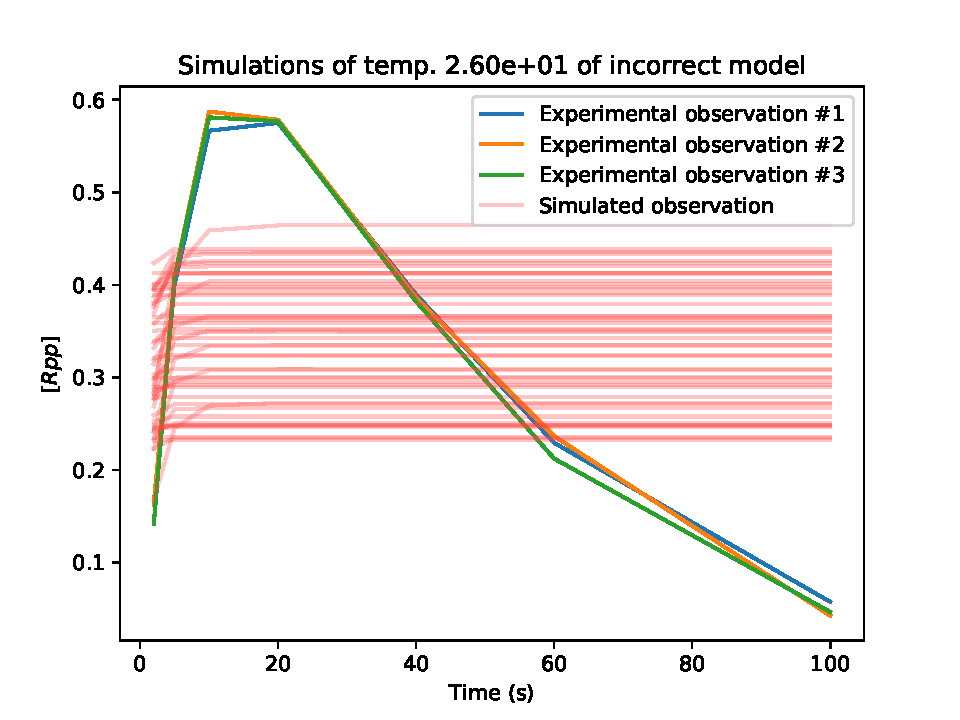
\includegraphics[clip=true,width=.45\linewidth]{experiments/abc_vs_snm/all_model/abc/msimulations_model3_25.pdf}
    \label{fig:girolami_model3_abc}}
&
    \subfigure[generalization model]{
    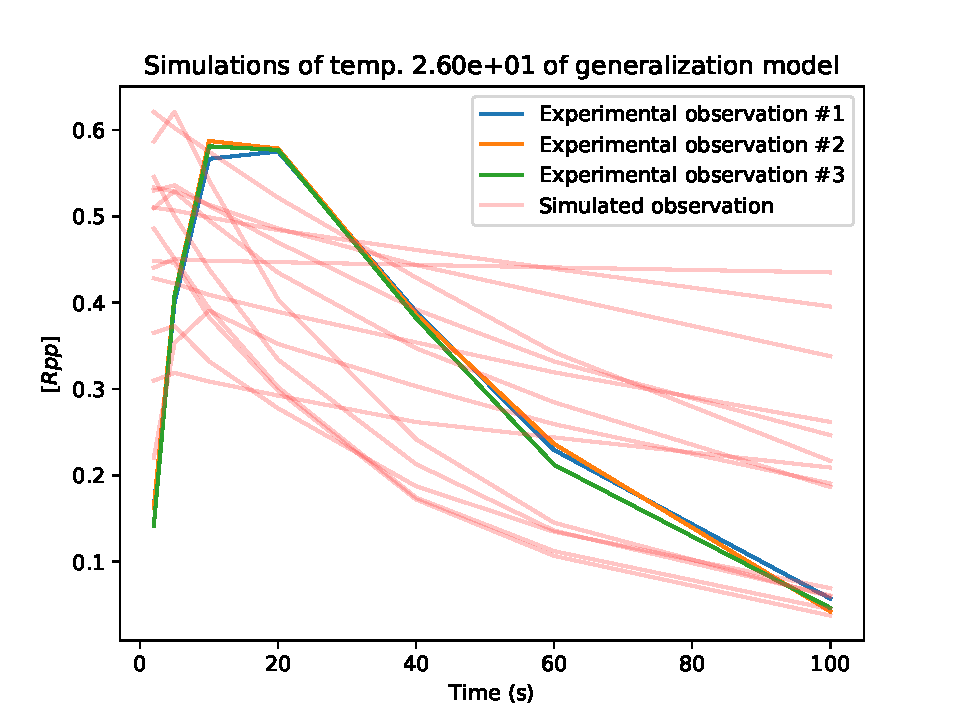
\includegraphics[clip=true,width=.45\linewidth]{experiments/abc_vs_snm/all_model/abc/msimulations_model4_25.pdf}
    \label{fig:girolami_model4_abc}}
    \end{tabular}
    \caption{The simulated dynamics of the four candidate models, using
    parameters generated on the ABC-SysBio software. There are 100
    individuals generated on each iteration of the algorithm, and each
    individual consists of a list of parameter values and a model
    indicator. Because of this, the number of produced simulations is 
    not equal between models, in fact, the better the fit of a model,
    the higher the number of individuals representing such model, and
    therefore, the higher the number of simulations shown. Each red line
    represent an individual simulation, and stronger red lines represent
    overlapping simulations. Lines with blue, yellow and green color
    represent experimental observations.}
    \label{fig:girolami_allmodel_abc}
\end{figure}

On figure~\ref{fig:girolami_allmodel_snm} we present the dynamics of a 
subset of parameters of the posterior distribution (or power posterior 
of $\beta = 1$), for all four candidate models. We can see on this
figure that SigNetMS could not find parameter values that allow the
incorrect model to reproduce experimental observations, which is
expected, and that the three other models candidate models could
closely reproduce the experimental observations. It is also interesting
to observe the dynamics produced by sampled parameters for other values
of $\beta$, which is shown on figure~\ref{fig:girolami_model1_progression_snm},
for the correct model only. Remember that from $\beta = 0$ to 
$\beta = 1$, a sequence of power posterior distributions is constructed 
by SigNetMS, bridging the prior and posterior distributions.

\begin{figure}[ht]
    \centering
    \begin{tabular}{c c}
    \subfigure[correct model]{
    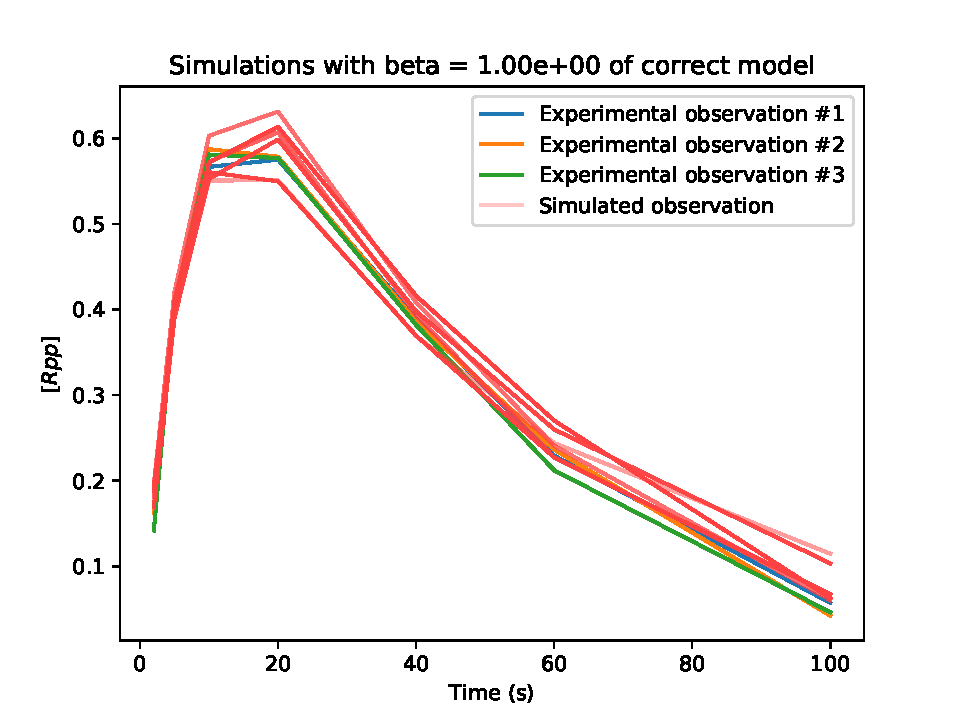
\includegraphics[clip=true,width=.45\linewidth]{experiments/abc_vs_snm/all_model/snm/msimulations_model1_39.pdf}
    \label{fig:girolami_model1_snm}}
    &
    \subfigure[simplified model]{
    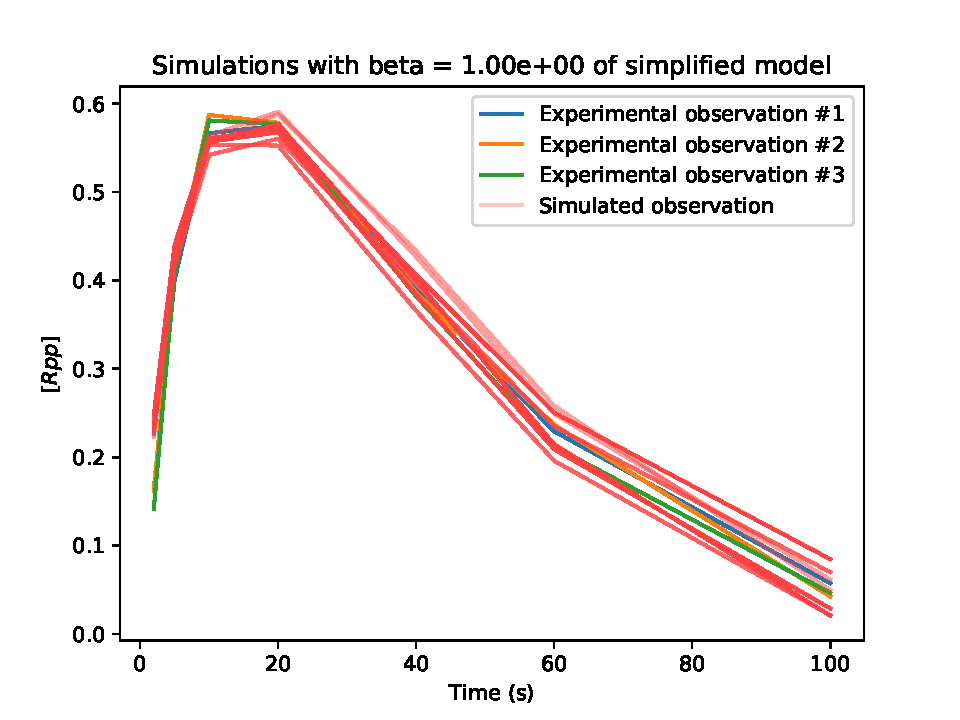
\includegraphics[clip=true,width=.45\linewidth]{experiments/abc_vs_snm/all_model/snm/msimulations_model2_39.pdf}
    \label{fig:girolami_model2_snm}} 
    \\
    \subfigure[incorrect model]{
    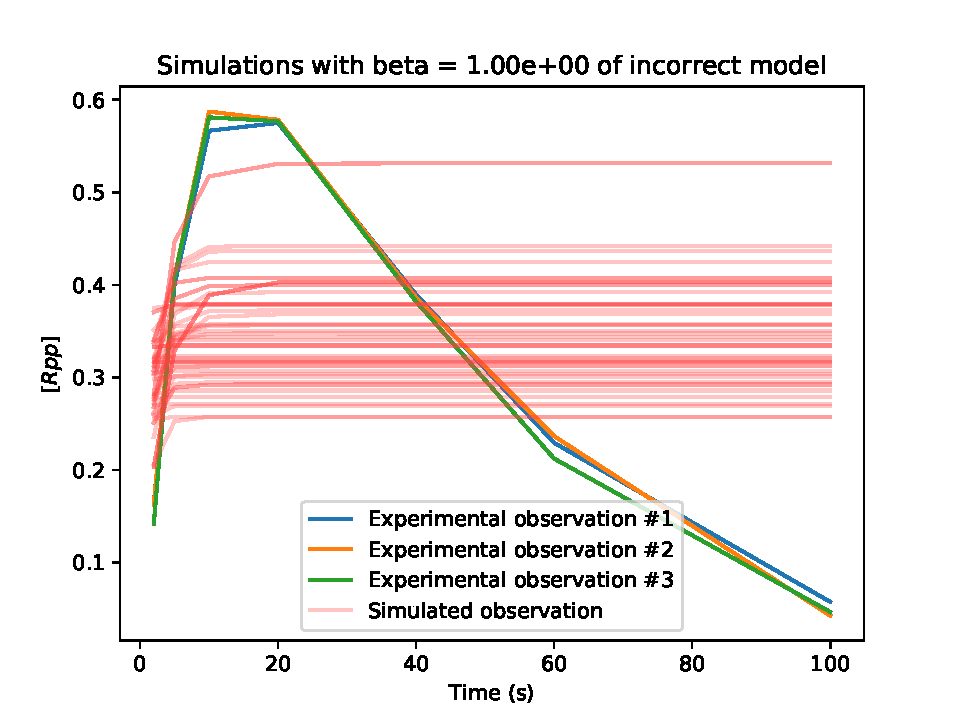
\includegraphics[clip=true,width=.45\linewidth]{experiments/abc_vs_snm/all_model/snm/msimulations_model3_39.pdf}
    \label{fig:girolami_model3_snm}}
&
    \subfigure[generalization model]{
    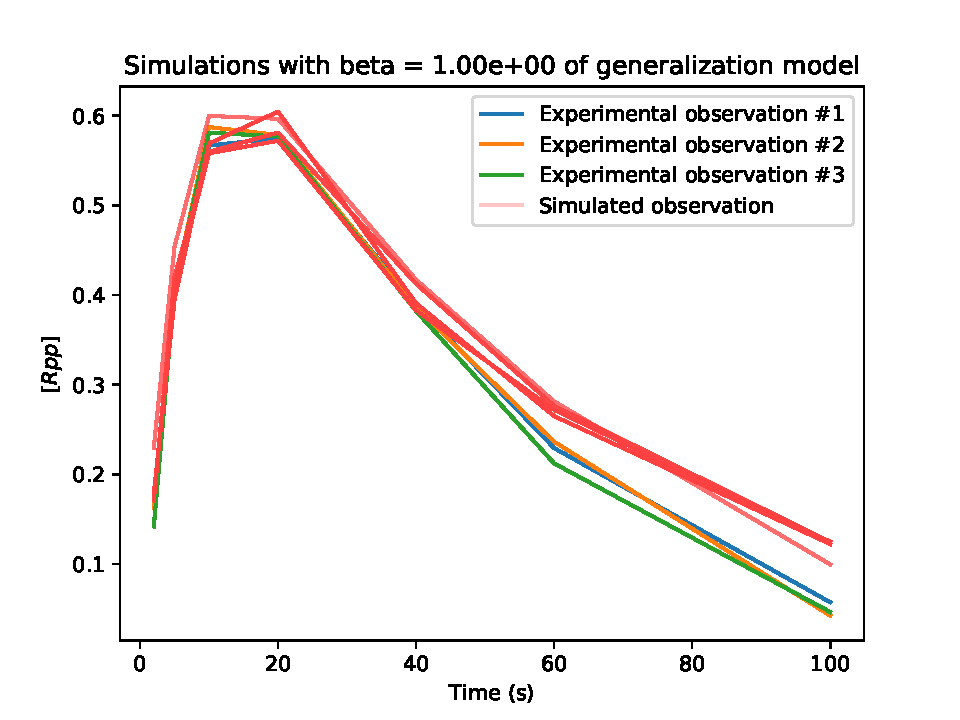
\includegraphics[clip=true,width=.45\linewidth]{experiments/abc_vs_snm/all_model/snm/msimulations_model4_39.pdf}
    \label{fig:girolami_model4_snm}}
    \end{tabular}
    \caption{The simulated dynamics of the four candidate models, using
    randomly chosen subsets of parameters from the sample produced by
    SigNetMS of the power posterior distribution of $\beta = 1$, which
    is the posterior distribution of parameters, $p({\bm \theta} | M,
    {\bm D})$. Red translucent lines represent the simulated dynamics, 
    using the sampled parameters, and stronger lines represent
    overlapping simulations. Lines with blue, yellow, and green color
    represent experimental observations.}
    \label{fig:girolami_allmodel_snm}
\end{figure}

\begin{figure}[ht]
    \centering
    \begin{tabular}{c c}
    \subfigure{
    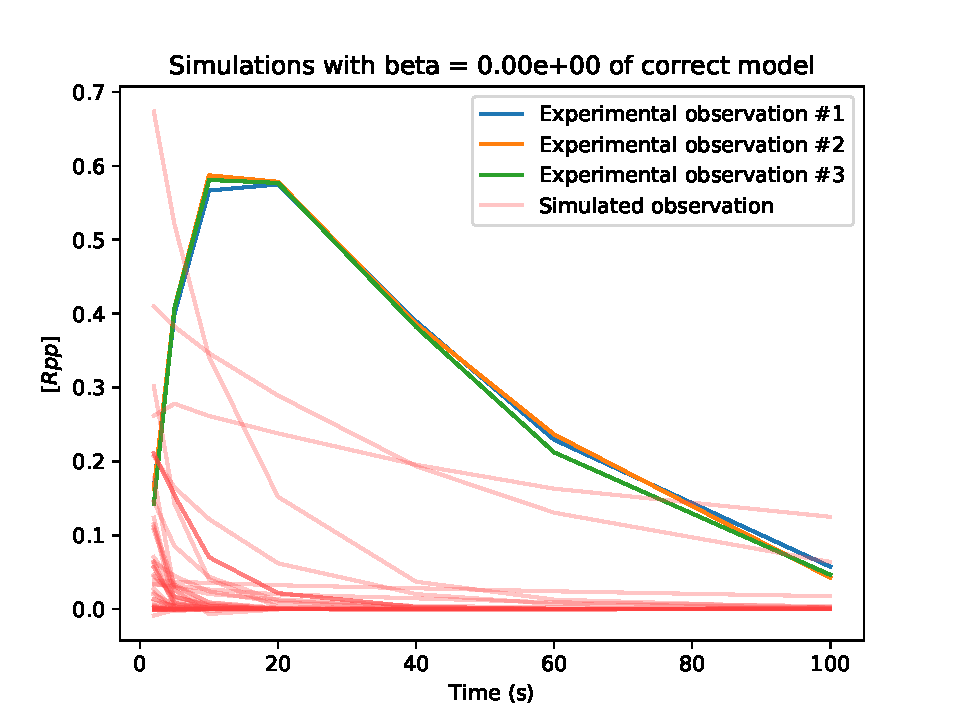
\includegraphics[clip=true,width=.45\linewidth]{experiments/abc_vs_snm/all_model/snm/msimulations_model1_0.pdf}
    \label{fig:girolami_model1_0_snm}}
    &
    \subfigure{
    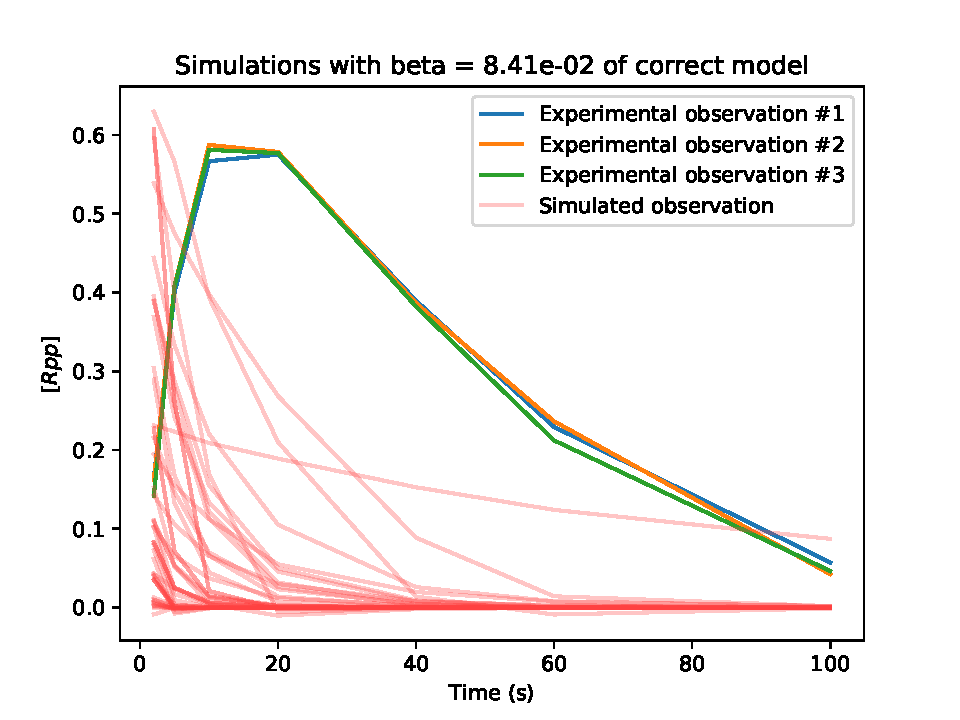
\includegraphics[clip=true,width=.45\linewidth]{experiments/abc_vs_snm/all_model/snm/msimulations_model1_21.pdf}
    \label{fig:girolami_model1_1_snm}} 
    \\
    \subfigure{
    \includegraphics[clip=true,width=.45\linewidth]{experiments/abc_vs_snm/all_model/snm/msimulations_model1_25.pdf}
    \label{fig:girolami_model1_2_snm}}
&
    \subfigure{
    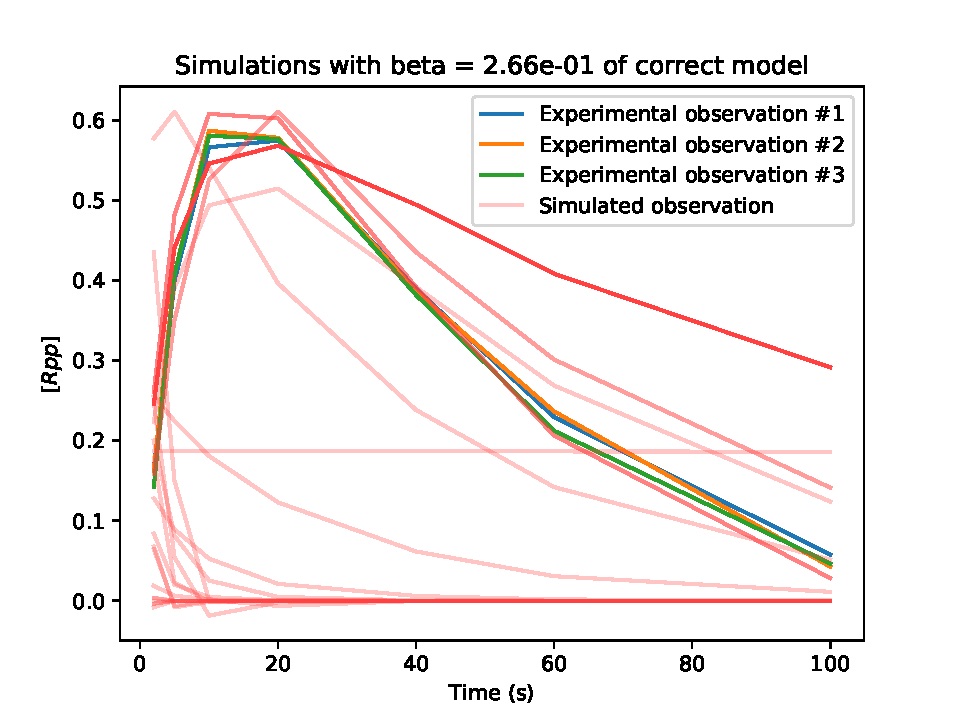
\includegraphics[clip=true,width=.45\linewidth]{experiments/abc_vs_snm/all_model/snm/msimulations_model1_28.pdf}
    \label{fig:girolami_model1_3_snm}}
    \\
    \subfigure{
    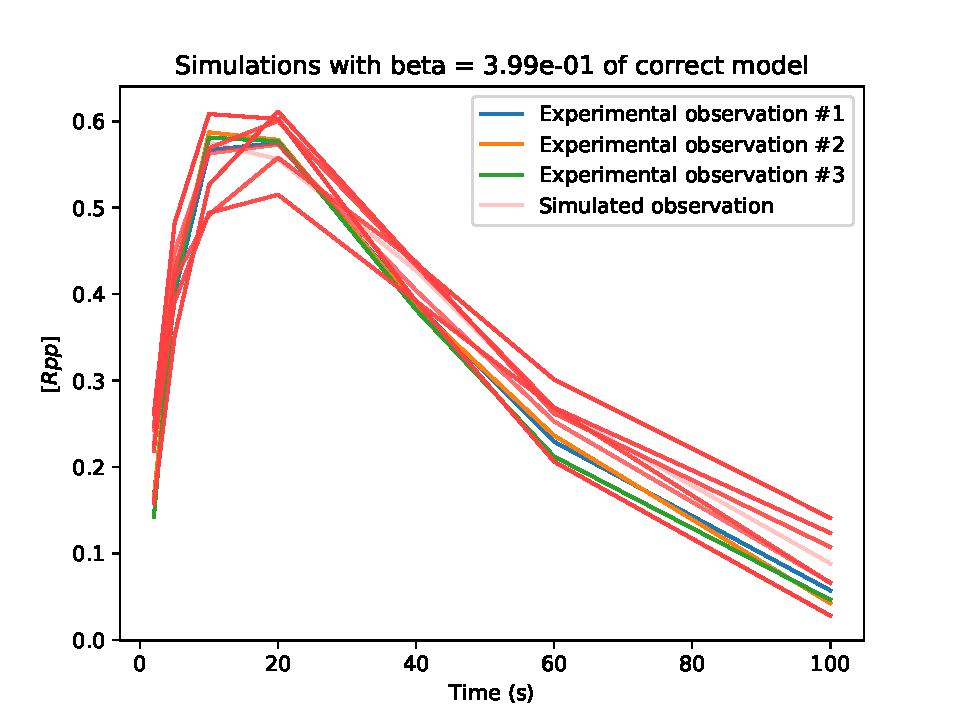
\includegraphics[clip=true,width=.45\linewidth]{experiments/abc_vs_snm/all_model/snm/msimulations_model1_31.pdf}
    \label{fig:girolami_model1_2_snm}}
&
    \subfigure{
    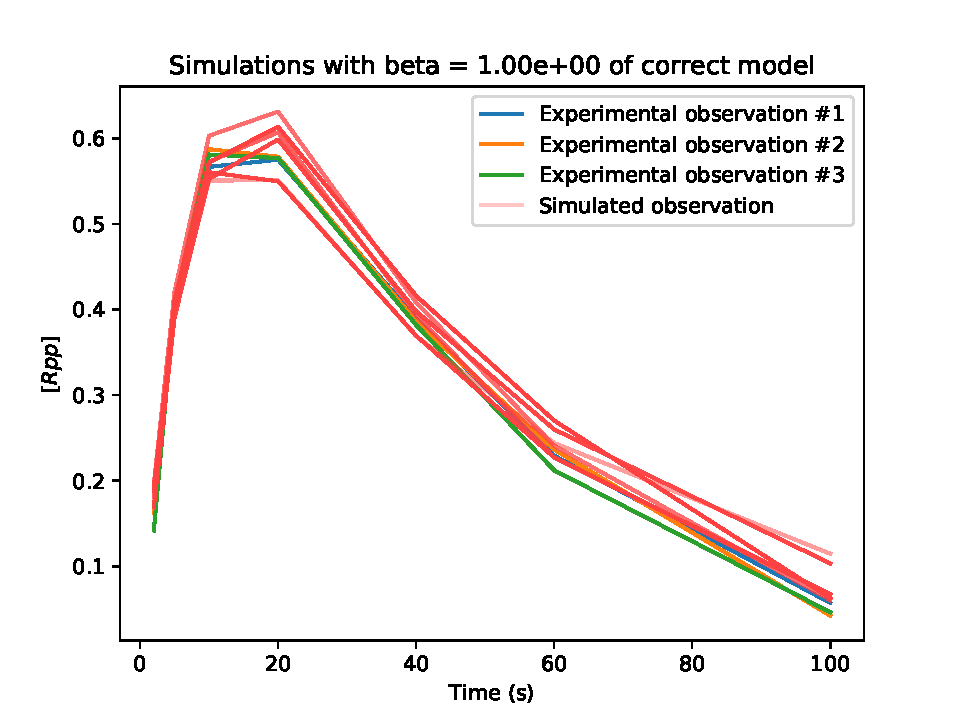
\includegraphics[clip=true,width=.45\linewidth]{experiments/abc_vs_snm/all_model/snm/msimulations_model1_39.pdf}
    \label{fig:girolami_model1_3_snm}}
    \end{tabular}
    \caption{The dynamics induced by samples of different power
    posterior distributions of parameters of the correct model. The
    value of $\beta$ increases from left to right and from top to
    bottom. We can observe how the curve of simulations progressively
    fits the curve of experimental observations.}
    \label{fig:girolami_model1_progression_snm}
\end{figure}

The ranking and the simulations indicate that SigNetMS is more
appropriate for our applications. To further investigate the results
produced by this software, we also created plots of approximations of
the produced power posterior samples, presented on 
figure~\ref{fig:girolami_model1_progression_snm}. These density function
estimates were created using the {\tt distplot} function of the Seaborn
Python package, which uses Gaussian Kernel Densinty Estimate (KDE) to
provide an estimation of the density function given a sample of such
distribution. The presented figure shows estimated power posterior
distributions, with different values of $\beta$, for the $k_1$ parameter
of the correct model, which had value $0.07$ when artificial
experimental data was created. We can see that as we increase the value 
of $\beta$, the posterior distribution concentrates on values around the
``true'' value of the parameter. It is also interesting to see that
although the estimated posterior is not necessarily centered on the 
``true'' value, the created simulations do approximate the experimental
observations.

\begin{figure}[ht]
    \centering
    \begin{tabular}{c c}
    \subfigure{
        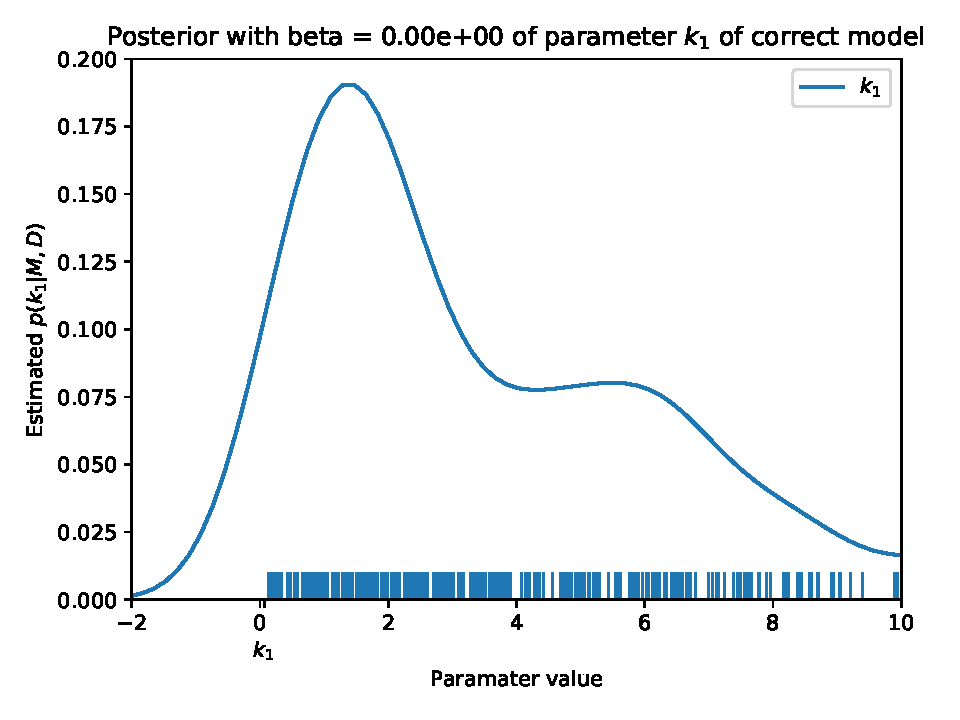
\includegraphics[clip=true,width=.45\linewidth]{experiments/abc_vs_snm/parameters_snm/model1_0_p0_k_1.pdf}
    \label{fig:girolami_model1_0_parameters}}
    &
    \subfigure{
    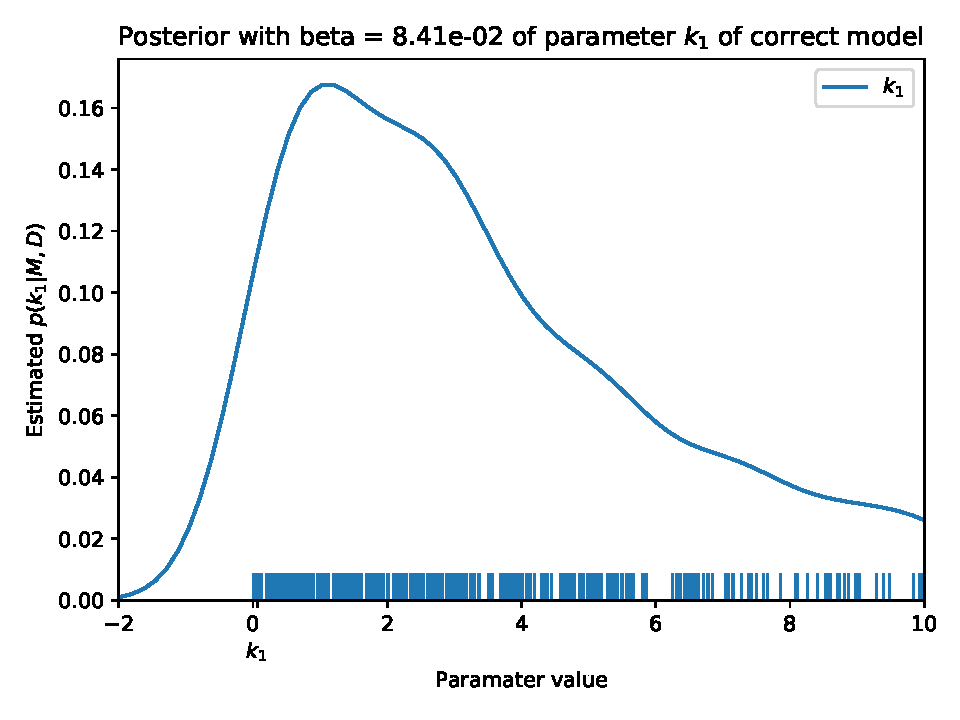
\includegraphics[clip=true,width=.45\linewidth]{experiments/abc_vs_snm/parameters_snm/model1_21_p0_k_1.pdf}
    \label{fig:girolami_model1_1_parameters}} 
    \\
    \subfigure{
    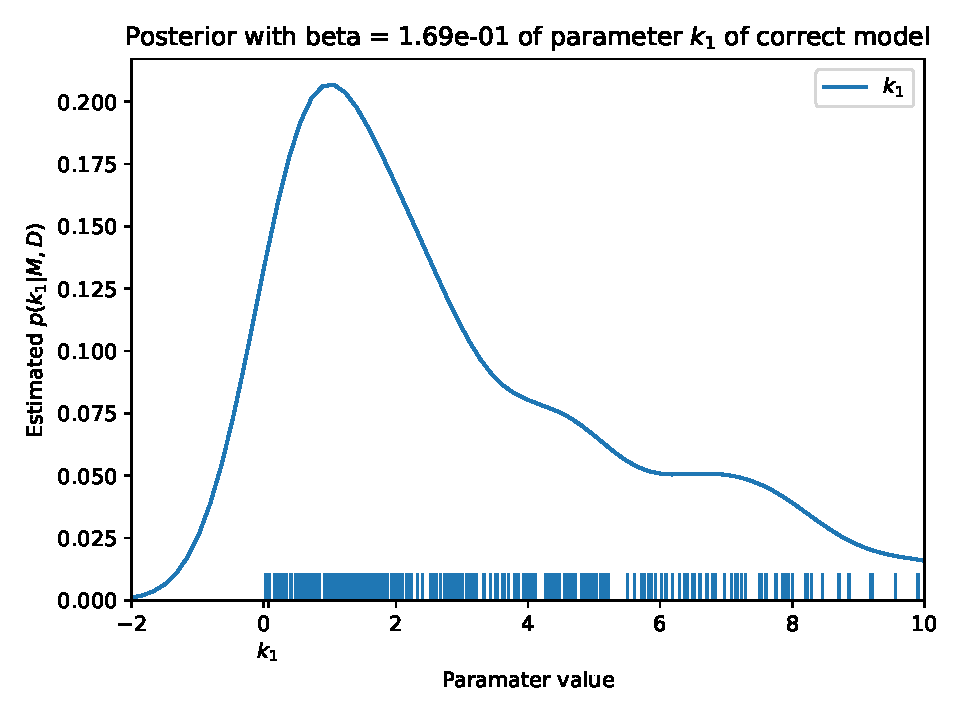
\includegraphics[clip=true,width=.45\linewidth]{experiments/abc_vs_snm/parameters_snm/model1_25_p0_k_1.pdf}
    \label{fig:girolami_model1_2_parameters}}
&
    \subfigure{
    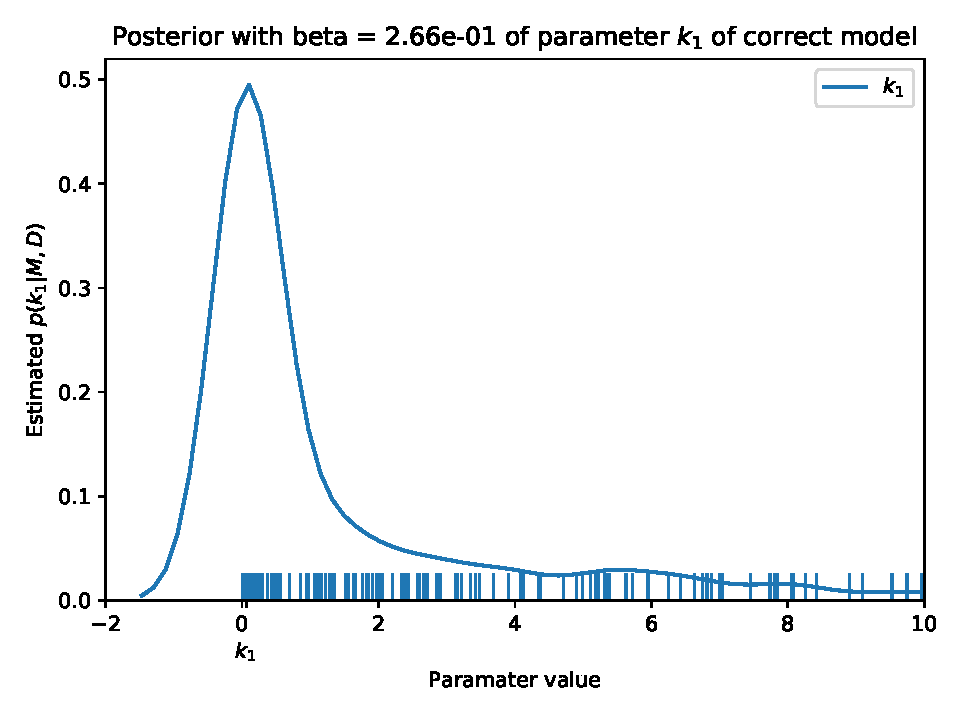
\includegraphics[clip=true,width=.45\linewidth]{experiments/abc_vs_snm/parameters_snm/model1_28_p0_k_1.pdf}
    \label{fig:girolami_model1_3_parameters}}
    \\
    \subfigure{
    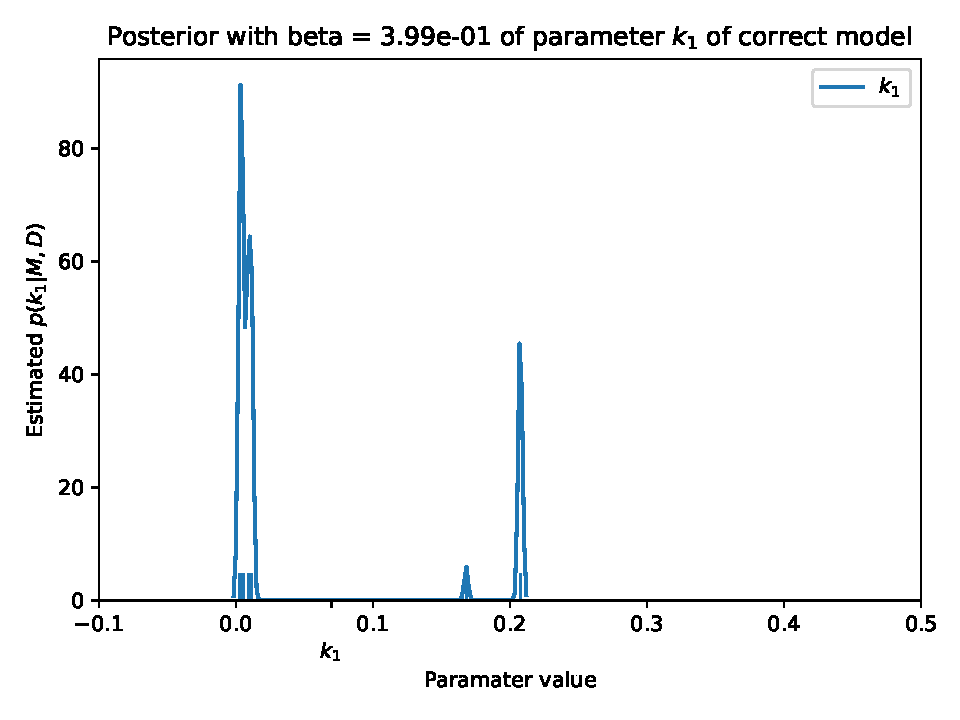
\includegraphics[clip=true,width=.45\linewidth]{experiments/abc_vs_snm/parameters_snm/model1_31_p0_k_1.pdf}
    \label{fig:girolami_model1_2_parameters}}
&
    \subfigure{
    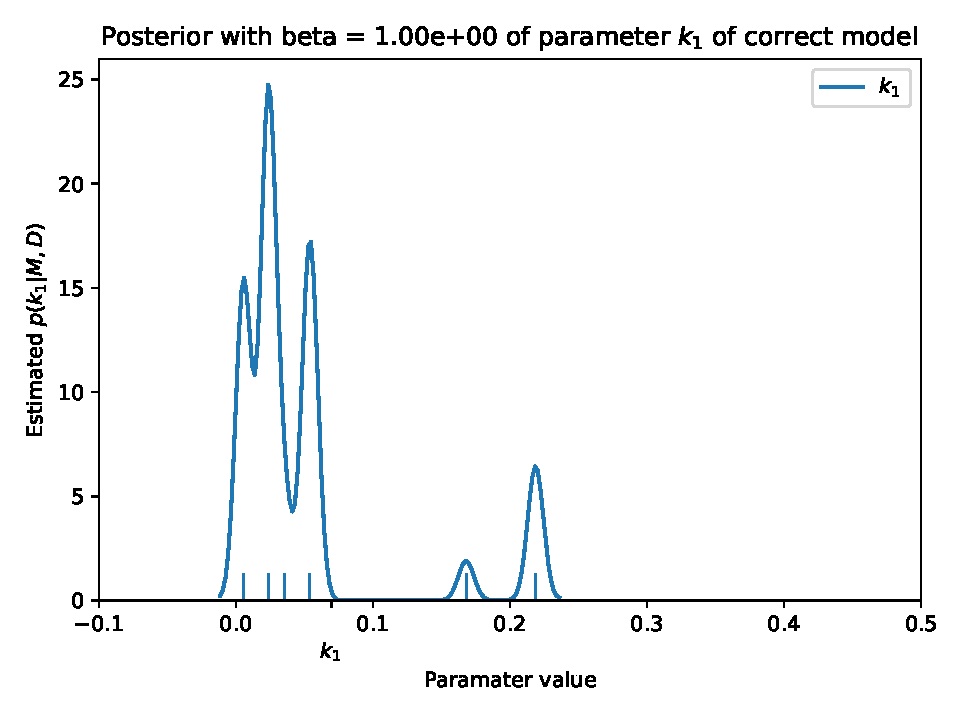
\includegraphics[clip=true,width=.45\linewidth]{experiments/abc_vs_snm/parameters_snm/model1_39_p0_k_1.pdf}
    \label{fig:girolami_model1_parameters}}
    \end{tabular}
    \caption{Approximation of the power posterior distribution of the 
    samples created by SigNetMS of parameter $k_1$ of the correct model.
    We show on this graph the estimated distribution of six different
    power posteriors, with increasing value of $\beta$ from left to
    right, from top to bottom. The approximation of this graph is
    created using {\tt distplot} function of Seaborn package. The value
    used for this parameter on the creation of the experimental data is
    $0.07$, and it is represented on the axis of the plots.}
    \label{fig:girolami_model1_progression_snm}
\end{figure}

\clearpage
\section{Model Selection as a Feature Selection Problem}
% After defining that SigNetMS is our software choice for model
% selection, we will construct another model selection problem instance.
% This time, we intend to use such instance to evaluate the approach
% of solving a model selection problem as a feature selection problem,
% with a Bayesian cost function. Although the instance we use is still 
% small, we will be able to access the surface of possible solutions and 
% get hints of how this surface is induced by the cost function we
% chose.
After defining that SigNetMS is our software choice for model selection,
we are now able to experiment and analyze the approach of solving a 
model selection problem as a feature selection problem, using a Bayesian
approach to define a cost function. To accomplish this, we created
another simple instance of model selection. Although this instance is
still a toy model, we will be able to access the space of possible
solutions and get a glance of the cost surface induced by SigNetMS over
this space.

A feature selection instance can be defined by a pair $(S, c)$ where $S$
is a set of features and $c$ is a cost function that evaluates subsets
of $S$. The space of solution is usually the power set of $S$,
$\mathcal{P}(S)$, and the cost function usually takes values from this 
space to positive real values, $c: \mathcal{P}(S) \to \fieldR$. An
optimal solution is a subset $X \in \mathcal{P}(S)$ such that $c(X) \leq
c(Y), \forall Y \in \powerset (S)$, however, it is important to notice
that the size of the search space grows exponentially with the number of
features and, in practice, with time consuming cost functions, it is
computationally unfeasible use optimal search algorithms. That is
exactly our case, since the cost function we propose to use, based on
SigNetMS, depends on the estimation of multiple power posteriors of
parameters and includes numerous numerical integrations of a system of
ordinary differential equations.

It is often useful to represent the search space with a boolean lattice, 
which is defined by the power set $\mathcal{P}(S)$ and the partial order 
relation $\subseteq$. More than an aid to represent the search space,
the boolean lattice provides a structure that is useful for search
algorithms to define paths and to take advantage of surface of the 
search space, as it is done on algorithms for the U-Curve problem, a 
special case of the feature selection problem where the cost function 
describes a u-shaped curve on every chain of the boolean lattice. The
U-Curve problem is still an NP-hard problem as the feature selection
problem is~\cite{Rei12}, however there are heuristics and optimal
algorithms that can be used on the U-Curve problem to produce a quality
answer (optimal or close to be optimal) with a feasible computational
time. Moreover, one can produce good results using U-Curve algorithms to 
solve a feature selection instance that is not necessarily U-Curve, but
does reproduce u-shaped curves with a few oscillations on chains of the
search space.

In our application, we are going to convert a model selection problem
into a feature selection problem. To do so, we define a set of candidate
reactions $S$ and a base model. Then, we consider that a set of feature
$X \in \powerset (S)$ represents a candidate model composed by the base
model plus the reactions from $X$. The cost function we use is the
logarithm of the marginal likelihood produced by SigNetMS.
Figure~\ref{fig:feature_selection_model_selection} shows an example of
feature selection instance that represents a model selection instance.

\begin{figure}[h!]
\begin{center}
    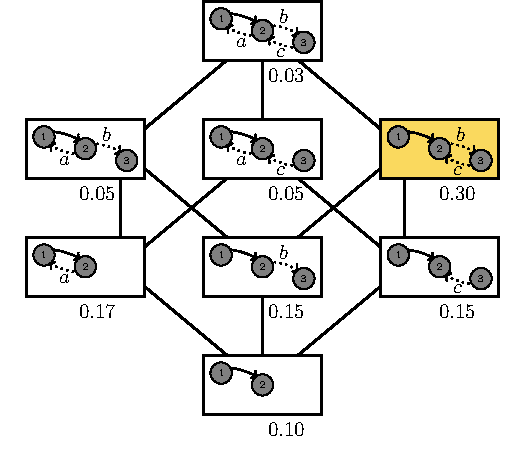
\includegraphics[width=1\textwidth]{experiments/Boolean_lattice_model_selection.pdf}
    \caption{A diagram with the search space and costs of a feature 
    selection problem that represents a model selection problem. Each 
    rectangle represents a subset of the power set of features, were
    reactions from such subset are drawn with dots. Links between 
    rectangles represent the $\subseteq$ relation; that is, two 
    rectangles linked represent two subsets of reactions $X$ and $Y$ 
    such that $X \subseteq Y$ (or $Y \subseteq X$). The set of features 
    is composed by three reactions, $\{a, b, c\}$, inducing the search 
    space with eight elements. The base model is composed by two 
    chemical species, $1$ and $2$ and a reaction between those species, 
    we can see this model at the base of the diagram, on the rectangle 
    that represents the empty set (no reaction are drawn with dots). 
    Each rectangle also represents a candidate model, which is composed 
    by the base model plus the reactions drawn with dots. The number
    below each rectangle represents the score (minus one times the cost)
    of each model. The optimal subset is drawn in yellow and it the
    subset of reactions $\{b, c\}$. Note that this instance is a U-Curve 
    instance, if we consider the cost as minus one times the score: for 
    every chain of rectangles, the cost of the model describes a u 
    shaped curve. As an instance, consider the chain $\emptyset, \{c\} 
    , \{a, c\}, \{a, b, c\}$, which has respectively the costs of
    $-0.10$, $-0.15$, $-0.30$, and $-0.03$.}
    \label{fig:feature_selection_model_selection}
    \end{center}
\end{figure}

After defining the feature selection instance, we will traverse the
search space in two ways. First, we will traverse chains from the empty
set to the complete set, to understand the shape of the cost function as
we increase the number of reactions. Then, we will run the Sequential 
Forward Search algorithm, a heuristic for the feature selection problem,
to try to find a good solution for our model selection problem.


% talk about search algorithms
% talk about the U-Curve problem  

% introduce an example of the boolean lattice

% The feature selection problem is...
% the features are blah,
% the cost function is bleh,

\subsection{Defining the Feature Selection Instance}
% The instance we chose to show is a Ras switch pathway. This pathway...
% This time we also define the correct model, which is shown on Figure.
% We define the space of features as the set of reactions shown on
% Figure.

% We define as a "base model", a simple pathway which has no reactions,
% and for each node of the search space, we consider that such node
% represents the empty model with the reactions present on that node.

% The list of candidate reactions is shown on figure blah
% 

The instance we prepared is based on a Ras switch pathway. Ras
represents a family of proteins that are common on signaling pathways
that participate on cell growth and differentiation. Because of this
participation, Ras proteins that are constantly switched on can play a 
part on some types of cancer. The model we consider for generating 
experiments, which we also call the ``correct'' model is shown on 
Figure~\ref{fig:ras_switch:correct_model}. This model shows a pathway
that decides the state of a Ras protein as switched on, represented by
RasGTP, and as switched off, represented by RasGDP. Five other chemical
species are present on this model, and they have the following initial
concentration: 200 for SOS; 0 for SOS\_allo\_RasGDP and
SOS\_allo\_RasGTP; 900 for RasGDP; 100 for RasGTP; 200 for GEF; and 125
for GAP. Once again, we omit concentration and reaction rate units for
the sake of simplificty. These chemical species interact in eight
different chemical reactions:
\begin{itemize}
    \item{$\ce{SOS + RasGDP ->[k2] SOS\_allo\_RasGDP}$};
    \item{$\ce{SOS\_allo\_RasGDP ->[d2] SOS + RasGDP}$};
    \item{$\ce{SOS + RasGTP ->[k1] SOS\_allo\_RasGTP}$};
    \item{$\ce{SOS\_allo\_RasGTP ->[d1] SOS + RasGTP}$};
    \item{$\ce{RasGTP -> RasGDP}$}, with SOS\_allo\_RasGTP as a
        catalyst, and $k3cat$ and $K3m$ as catalytic constant and
        Michaelis constant, respectively;
    \item{$\ce{RasGTP -> RasGDP}$}, with SOS\_allo\_RasGDP as a 
        catalyst, and $k4cat$ and $K4m$ as catalytic constant and
        Michaelis constant, respectively;
    \item{$\ce{RasGTP -> RasGDP}$}, with GEF as a catalyst, and
        $k6cat$ and $K6m$ as catalytic constant and Michaelis constant,
        respectively;
    \item{$\ce{RasGDP -> RasGTP}$}, with GAP as a catalyst, and
        $k5cat$ and $K5m$ as catalytic constant and Michaelis constant,
        respectively.
\end{itemize}

\begin{figure}[H]
\begin{center}
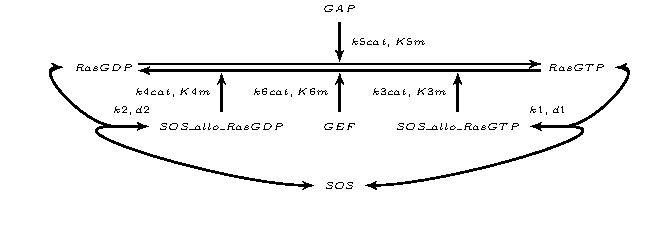
\includegraphics[width=1\textwidth]{experiments/ras_switch/correct.pdf}
\caption{A representation of a Ras switch pathway that we consider as
    the correct model for our model selection experiment. This model
    contains seven chemical species, and eight different chemical
    reactions. Reversible reactions are represented with arrows poiting
    both directions, with reaction rate parameters over the reaction,
    with the forward reaction parameter first and then the parameter of
    the reverse reaction. Michaelis-Menten reactions are represented
    with parameters to the left of the arrow from starting at the
    enzyme, with the catalystic parameter first, and then the Michaelis
    constant.
}
\label{fig:ras_switch:correct_model}
\end{center}
\end{figure}

We used this model to generate an artificial experiment where the
concentration of activated Ras was measured at the time steps of 30,
60, 90, 120, 150, 180, 210, and 240 seconds.
Figure~\ref{fig:ras_switch:experimental_observations} shows a graph of
such experimental measurements. Similarly to the experiment of the 
previous section, those observations were created by simulating the 
correct model and then adding a Gaussian error of mean zero and standard
deviation of 0.01. The reaction rate parameters used to create these
simulations are: k1 $= 1.8e-4$, d1 $= 3$, k2 $= 1.7e-4$, d2 $=0.04$,
k3cat $= 3.8$, K3m $=1.64e3$, k4cat $= 0.003$, K4m $= 9.12e3$, k5cat
$= 0.1$, K5m $= 1.07e2$, k6cat $= 0.01$, and K6m $=1836$ (once again,
remember that we are omitting units for the sake of simplicity).
%<parameter id="k1"    value="1.8e-4"/>
%<parameter id="d1"    value="3.0"/>
%<parameter id="k2"    value="1.7e-4"/>
%<parameter id="d2"    value="0.04"/>
%<parameter id="k3cat" value="3.8"/>
%<parameter id="K3m"   value="1.64e3"/>
%<parameter id="k4cat" value="0.003"/>
%<parameter id="K4m"   value="9.12e3"/>
%<parameter id="k5cat" value="0.1"/>
%<parameter id="K5m"   value="1.07e2"/>
%<parameter id="k6cat" value="0.01"/>
%<parameter id="K6m"   value="1836"/>

\begin{figure}[H]
\begin{center}
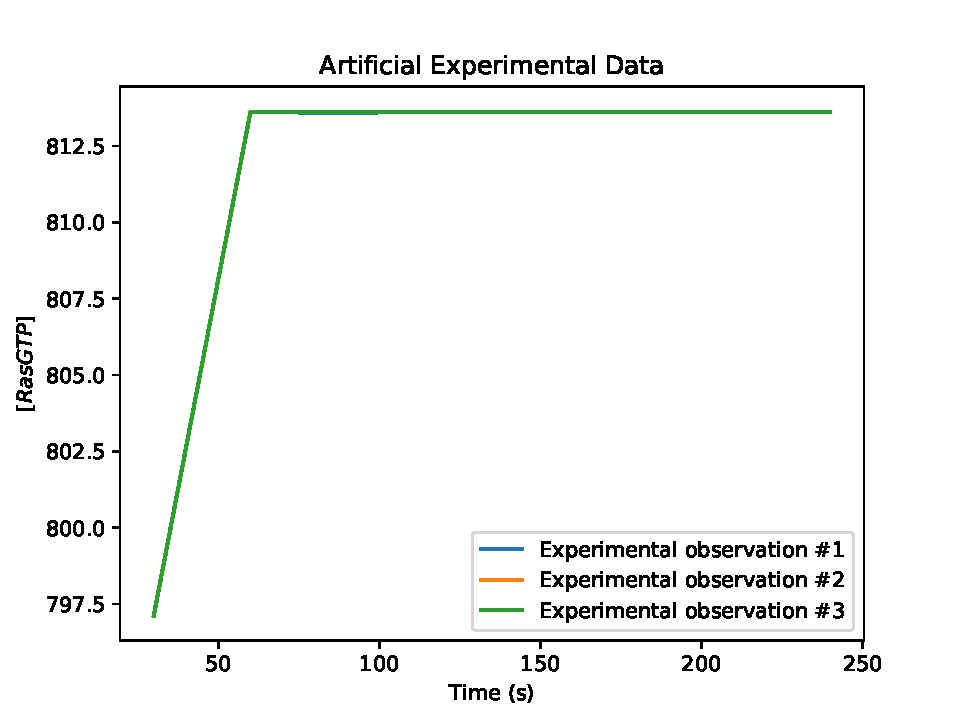
\includegraphics[width=.75\textwidth]{experiments/ras_switch/experiment_plot.pdf}
\caption{Experimental data generated with our correct model for the Ras
    switch pathway. There is a set of three observations being
    represented, however, the time points observations of [RasGTP] are
    close enough that the lines of each experiment overlap. The time
    points considered are 30, 60, 90, 120, 150, 180, 210, and 240
    seconds; the lines are produced with a linear interpolation of
    measurements on these points.}
\label{fig:ras_switch:experimental_observations}
\end{center}
\end{figure}

To construct our search space, we considered as the base of our search
space a trivial model, containing no reactions. For the set of features,
we considered all reactions from the correct model (i.e. the correct
model is present on the search space), plus two other reactions. A
complete list of candidate reactions is shown of
Figure~\ref{fig:ras_switch:features}. The complete list of candidate
reactions is saved in a JSON file, which also stores information about
rate parameters for each reaction, including its name and prior. In this
experiment we defined Uniform prior distributions, using our prior
knowledge about reactions. As a matter of fact, in our first approach we
used Gamma distributions, however, due to numerical instabilities we
decided Uniform distributions for its simplicity and restrictiveness.
({\color{blue}TODO: should I include prior distributions on the text?}) 

Figure~\ref{fig:ras_switch:features} also presents an arbitrary order we
choose for these reactions. This order, from (a) to (j) is useful to
enumerate points of the search space, something that search algorithms
can rely on when traversing the search space. With this order, we can
introduce the concept of characteristic vector, which is a vector
composed by boolean flags that represents a point of the search space,
and, that is, a subset of features. If the i-th element of the
characteristic vector is a 0, then the i-th feature is not present on 
the subset represented, if the i-th elemnt is 1, then this feature is
present on the subset. Considering the order we choose for this Ras
switch instance, we could say that the subset represented by the
characteristic vector 0101010001 has the reactions: SOS\_allo\_RasGDP
decomplexation, SOS\_allo\_RasGTP decomplexation, Ras activation by
SOS\_allo\_RasGTP, and GAP activation by RasGTP.

After defining our set of features, a base model, the rule for 
defining the model associated to a subset of features, and the cost
function, we are now able to experiment solving the model selection
problem as a feature selection problem. It is important to remember that
our cost function, the output of SigNetMS, is computationally expensive
and, since we have 10 features, the search space has the size $2^{10}$.
That makes it unfeasible to optimally search on the space, and therefore
we choose a heuristic to search for a good solution.


\begin{figure}[H]
    \centering
    \begin{tabular}{cc}
    \subfigure[SOS\_allo\_RasGDP complexation]{
        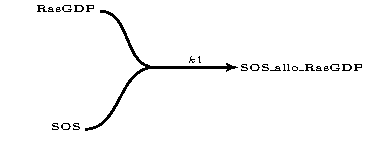
\includegraphics[clip=true,width=.35\linewidth]{experiments/ras_switch/reactions/sos_allo_rasgdp_complexation.pdf}
    }
    &
    \subfigure[SOS\_allo\_RasGDP decomplexation]{
        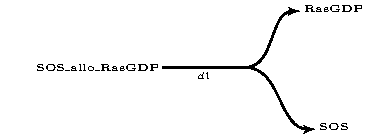
\includegraphics[clip=true,width=.35\linewidth]{experiments/ras_switch/reactions/sos_allo_rasgdp_decomplexation.pdf}
    }
    \\
    \subfigure[SOS\_allo\_RasGTP complexation]{
    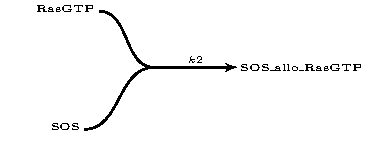
\includegraphics[clip=true,width=.35\linewidth]{experiments/ras_switch/reactions/sos_allo_rasgtp_complexation.pdf}
    }
    &
    \subfigure[SOS\_allo\_RasGTP decomplexation]{
    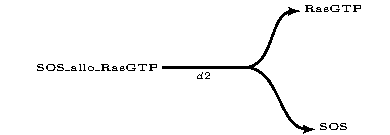
\includegraphics[clip=true,width=.35\linewidth]{experiments/ras_switch/reactions/sos_allo_rasgtp_decomplexation.pdf}
    }
    \\
    \subfigure[Ras inactivation by GAP]{
    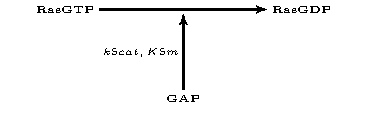
\includegraphics[clip=true,width=.35\linewidth]{experiments/ras_switch/reactions/ras_inactivation_by_gap.pdf}
    }
    &
    \subfigure[Ras activation by SOS\_allo\_RasGTP]{
    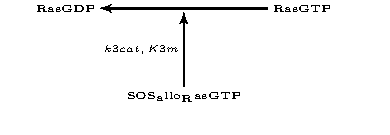
\includegraphics[clip=true,width=.35\linewidth]{experiments/ras_switch/reactions/ras_activation_by_sos_allo_RasGTP.pdf}
    }
    \\
    \subfigure[Ras activation by SOS\_allo\_RasGDP]{
    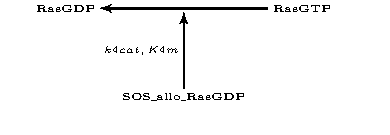
\includegraphics[clip=true,width=.35\linewidth]{experiments/ras_switch/reactions/ras_activation_by_sos_allo_RasGDP.pdf}
    }
    &
    \subfigure[Ras activation by GEF]{
    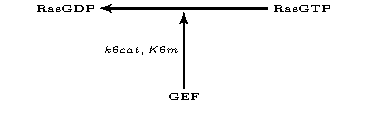
\includegraphics[clip=true,width=.35\linewidth]{experiments/ras_switch/reactions/ras_activation_by_GEF.pdf}
    }
    \\
    \subfigure[Ras activation by SOS]{
    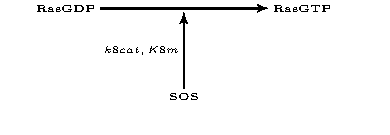
\includegraphics[clip=true,width=.35\linewidth]{experiments/ras_switch/reactions/ras_activation_by_SOS.pdf}
    }
    &
    \subfigure[GAP activation by RasGTP]{
    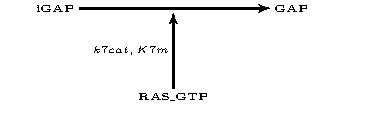
\includegraphics[clip=true,width=.35\linewidth]{experiments/ras_switch/reactions/gap_activation_by_RasGTP.pdf}
    }
    \end{tabular}
    \caption{All candidate reactions, or the set of features for our
    feature selection problem. Reactions (a) to (h) are all the
    reactions of the considered ``correct'' model.}
    \label{fig:ras_switch:features}
\end{figure}

% SFS experiment
\subsection{Using Sequential Forward Selection to Select a Model}
As discussed in the previous section, the feature selection instance we
have in hands has a search space and cost function that makes it
unfeasible to use an optimal algorithm of feature selection. Therefore,
we use the Sequential Forward Selection (SFS)~\cite{Whitney1971} 
heuristics to search for a solution.
% also want to talk about what we want to check in this experiment.
% With this experiment we will be able to analyze the solution given in
% our approach. We expect that we are able to at least find a model that
% correctly describes the dynamics observed on the experiments

The Sequential Forward Selection heuristics is a greedy algorithm that
starts with the empty set of features and then, for each iteration,
decides to add the ``best'' remaining feature to the current solution.
Although it is very easy to find instances in which this algorithm is
not optimal (including U-Curve instances), it can generally find  fairly
good solutions in many cases, making it a good choice to explore spaces
with unknown surfaces, such as in our case. Pseudocode~\ref{code:sfs}
presents the dynamics of the SFS heuristics.

% pseudo código
\begin{algorithm}[H]
\textsc{SFS} $(S, c)$
\begin{algorithmic}[1]
    \State $X \gets \emptyset$
    \State {\tt did\_impove} $\gets$ {\tt True}
    \While{{\tt did\_improve}}
        \State $s^* \gets NIL$
        \For{$s \in S$ and $s \notin X$}
            \If{$c(X \cup \{s\}) < c(X \cup \{s^*\})$}
                \State $s^* \gets s$
            \EndIf
        \EndFor
        \If{$s^*$ is $NIL$}
            \State {\tt did\_improve} $\gets$ {\tt False}
        \EndIf
    \EndWhile
    \Return $X$
\end{algorithmic}
\caption{A pseudocode representing the SFS algorithm.}
\label{code:sfs}
\end{algorithm}


% resultados e análise dos resultados
\subsubsection{Results of the search}
The SFS search was conduced in a server running with an Intel 
Xeon E5-2690 CPU, and 252GB of RAM memory. The total time to conduce the
experiment was about 26 hours, with 42 calls to the cost function, that
is, 42 points of the search space were visited. The chain of subsets the
algorithm traversed, from the base to the found solution, is shown on 
Table~\ref{tab:sfs_trace}.
% how long did it take do finish?
% want to talk about the chain produced

The best model found has the characteristic vector $0011010100$ and had 
the logarithm of the marginal likelihood of $10.8$. This model has the 
following reactions: SOS\_allo\_RasGTP complexation, SOS\_allo\_RasGTP
decomplexation, Ras activation by SOS\_allo\_RasGTP and Ras activation
by GEF.


\begin{table}[H]
\centering
\begin{tabular}{c|cll}
\hline
Characteristic Vector && \multicolumn{1}{l}{Score} &
\multicolumn{1}{l}{Cost function time (seconds)} \\
\hline
    0000000000 && 330721.05	& 669.79	\\
    0010000000 && 245681.93	& 889.42	\\
    0010010000 && 211.98	& 3408.28	\\
    0011010000 && 5.30,	& 2974.71	\\
    0011010100 && -10.89	& 3756.48	\\  
\hline
\hline
\end{tabular}
\caption{The trace of the SFS run on the Ras switch instance. The
    characteristic vector determines the set of reactions present on the
    model; the Score is minus one times the marginal likelihood of
    the model; and, the Cost function time is the total time used by 
    SigNetMS to calculate the marginal likelihood.}
\label{tab:sfs_trace}
\end{table}

Even though the resulting subset is not the correct model, the marginal
likelihood indicates that the model reasonably approximates the
experimental measurements. To verify this, we took the sample of the
posterior of model parameters produced by SigNetMS and created plots of 
simulations using those sampled parameters.
Figure~\ref{fig:ras_switch_solution} shows simulations created using
different power posterior samples. We can see that as $\beta$ increases,
the simulation approximates better the experimental results, to the
point where the simulation curves overlap with the experimental curves.
That indicates that, in fact, model $0011010100$ is able to reproduce
the dynamics observed on experimental observations.

\begin{figure}[ht]
    \centering
    \begin{tabular}{c c}
    \subfigure{
    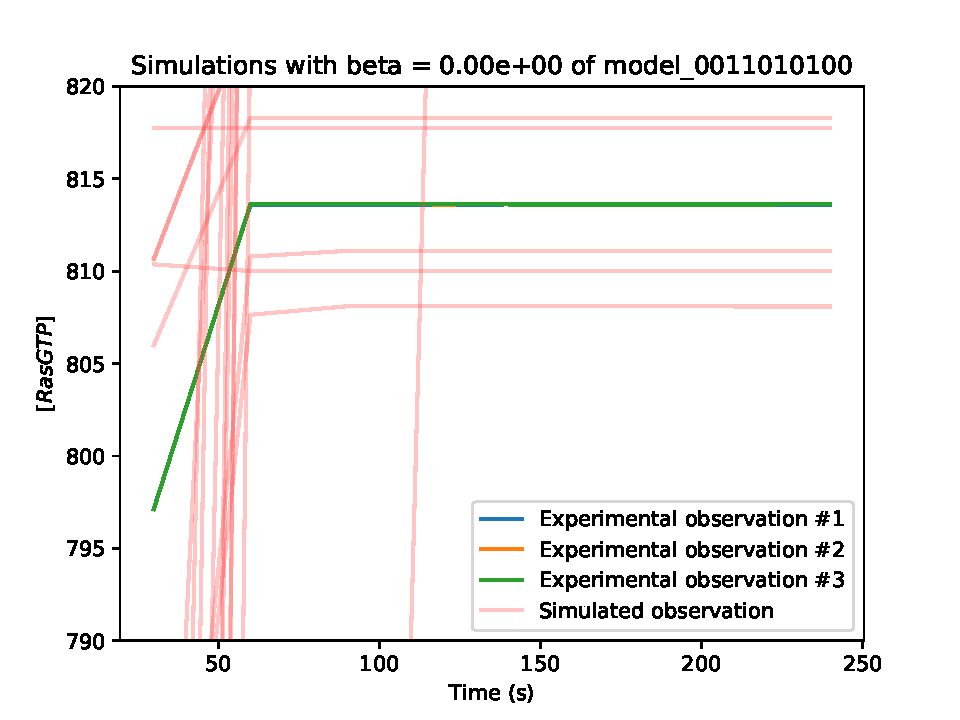
\includegraphics[clip=true,width=.45\linewidth]{experiments/ras_switch/simulations/msimulations_model_0011010100_0.pdf}}
    &
    \subfigure{
    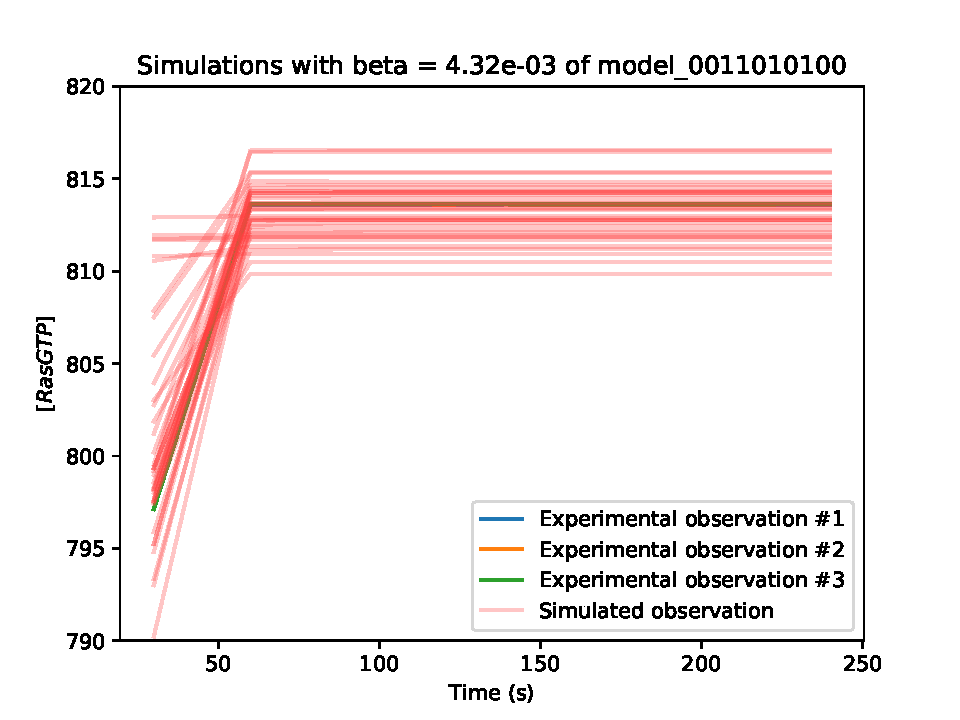
\includegraphics[clip=true,width=.45\linewidth]{experiments/ras_switch/simulations/msimulations_model_0011010100_10.pdf}}
    \\
    \subfigure{
    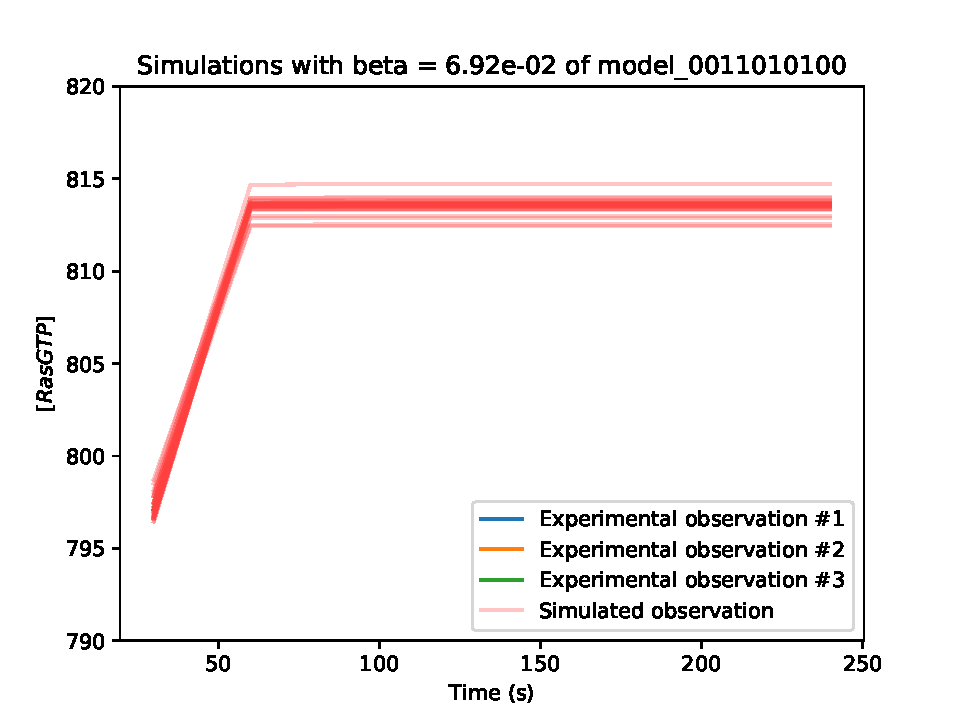
\includegraphics[clip=true,width=.45\linewidth]{experiments/ras_switch/simulations/msimulations_model_0011010100_20.pdf}}
    &
    \subfigure{
    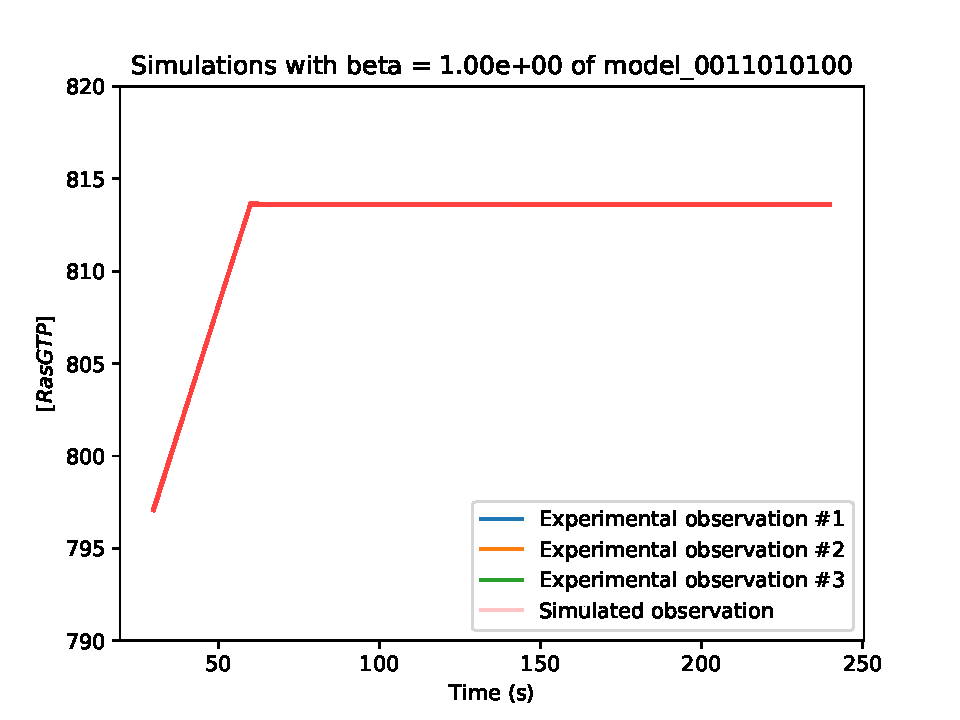
\includegraphics[clip=true,width=.45\linewidth]{experiments/ras_switch/simulations/msimulations_model_0011010100_39.pdf}}
    \\
    \end{tabular}
    \caption{Simulations created with power posterior samples of Ras
    switch model with characteristic vector $0011010100$, which is the
    model found by the SFS search. The model parameters used to create
    these simulations were sampled when the SFS algorithm evaluated the
    cost function for the model; when the cost function was called,
    SigNetMS produced both the estimation of the log of the marginal
    likelihood and samples of different power posteriors of model
    parameters. There were 40 different power posteriors sampled, and we
    show only four of them on this figure. Since the range of the plot
    area is fixed, it may seem that the first figure has less lines than
    the other ones; that only indicate that some simulations did not
    appear on the plot area.}
    \label{fig:ras_switch_solution}
\end{figure}



% show the cost of the correct model, and explain why it is not the
% optimal.

% Section: analyzing a chain of the feature space
% and that the optimal is not the best subset found
% however, we can see on figure blah that the found best subset does
% reproduce the experiments behaviour.

% maybe show how the optimal model scores?

% done!
